
% Application Features Chapter
% In this chapter all the features and objects of this application is explained
\subsection{Architecture of the Application}
\vspace{30mm}
  \begin{figure}[h!]
    \centering 
    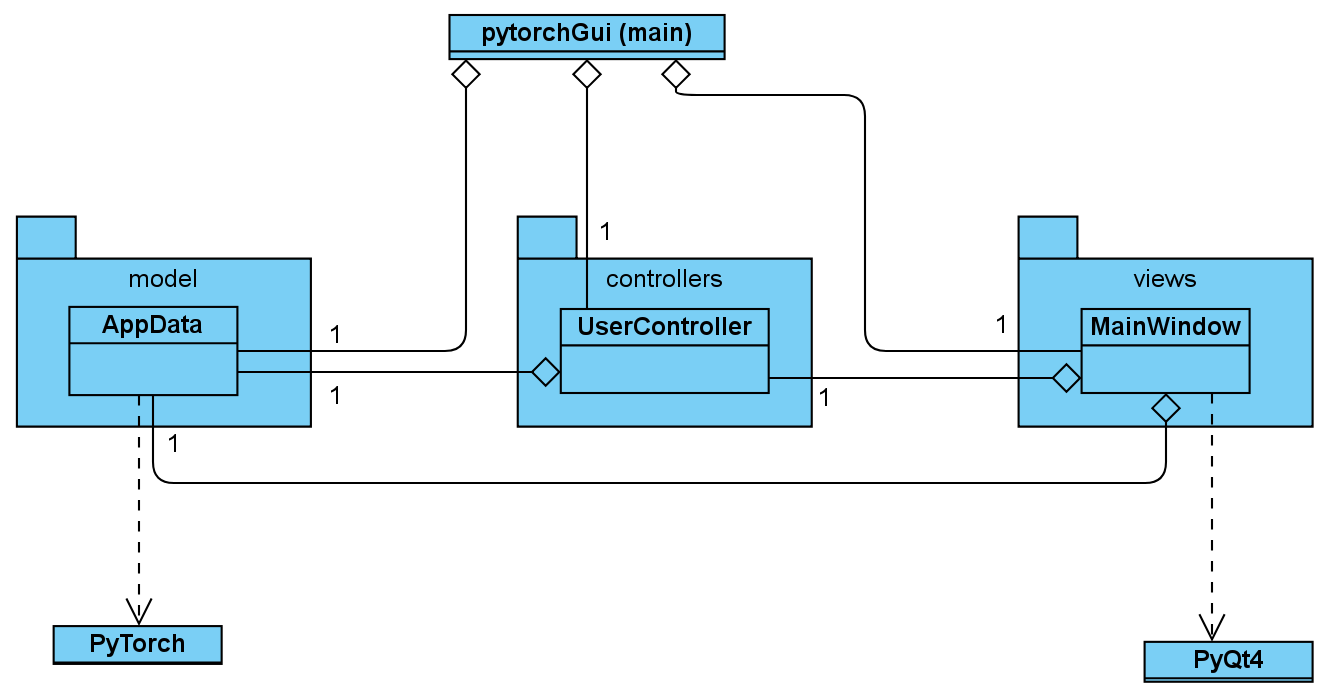
\includegraphics[scale=0.3]{figures/GlobalDiagram.png}
    \caption{Global architecture}
\end{figure}
\subsubsection{The MVC pattern}
Before we started to develop our application, we first had to choose a pattern to implement our functionalities. Since we are developing a graphical interface, we decided to implement one of the most commonly used pattern for this kind of application : \textbf{the MVC pattern}.
\newline MVC stands for \textbf{Model-View-Controller}. It means that the application is separated into three main packages :
\begin{itemize}
    \item The model : It contains all the logic and data of the application. It is independent from the interface, and we should be able to execute all of the program functionalities from here.
    \item The view : It contains the code of the graphical interface. There are widgets and modules used to pilot the application, and others to display results.
    \item The controller : It is responsible to do the link between the view and the model. It is called by the view when the user requires an action, it validates and transforms the data to make it fit to the model.
\end{itemize}

\textbf{Important note :} Our application does not strictly follow the MVC pattern. As a matter of fact, in a true MVC pattern, the view should not call the model directly, and should always go through the controller for every action. We found that it was quite heavy to implement in many cases. For example when the view needs a single value from the model, we found it was not necessary to call the controller. Thus, we also added a link between the view and the model, so that the view can call the model directly in those cases.

\begin{figure}[h!]
    \centering 
    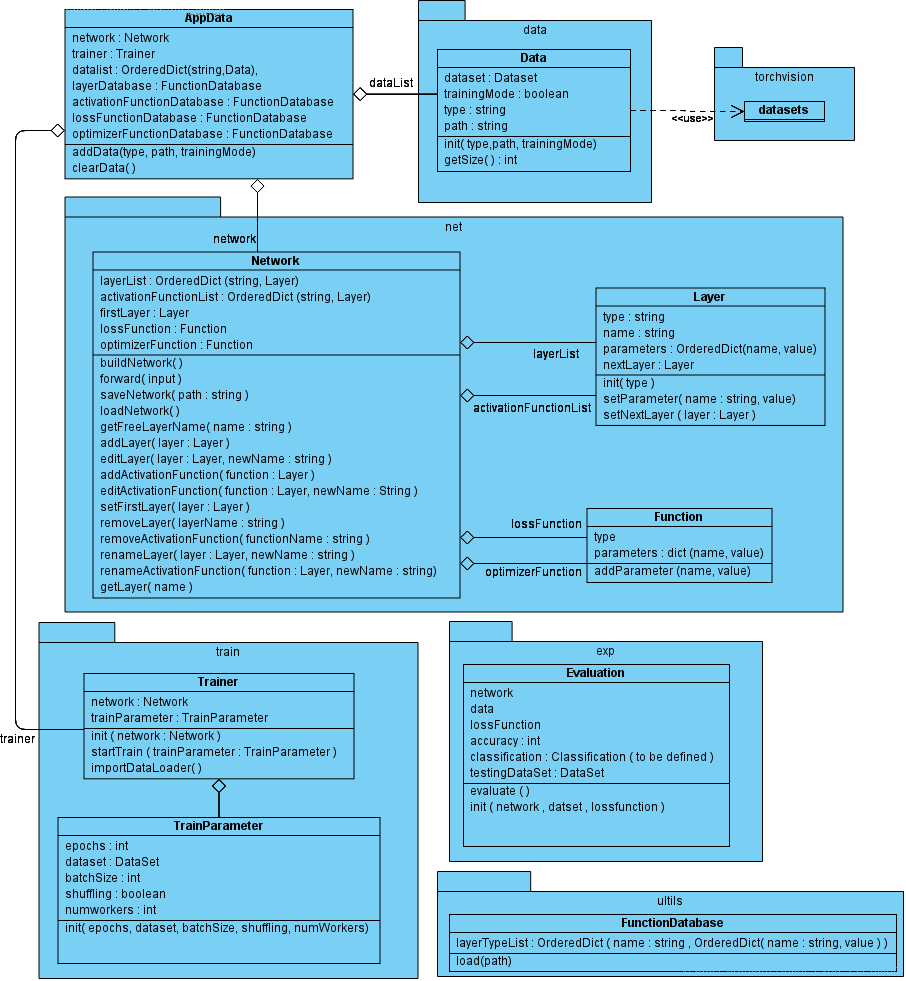
\includegraphics[scale=0.5]{figures/ModelDiagram.png}
    \caption{Model class diagram}
  \end{figure}
  
\begin{figure}[h!]
    \centering 
    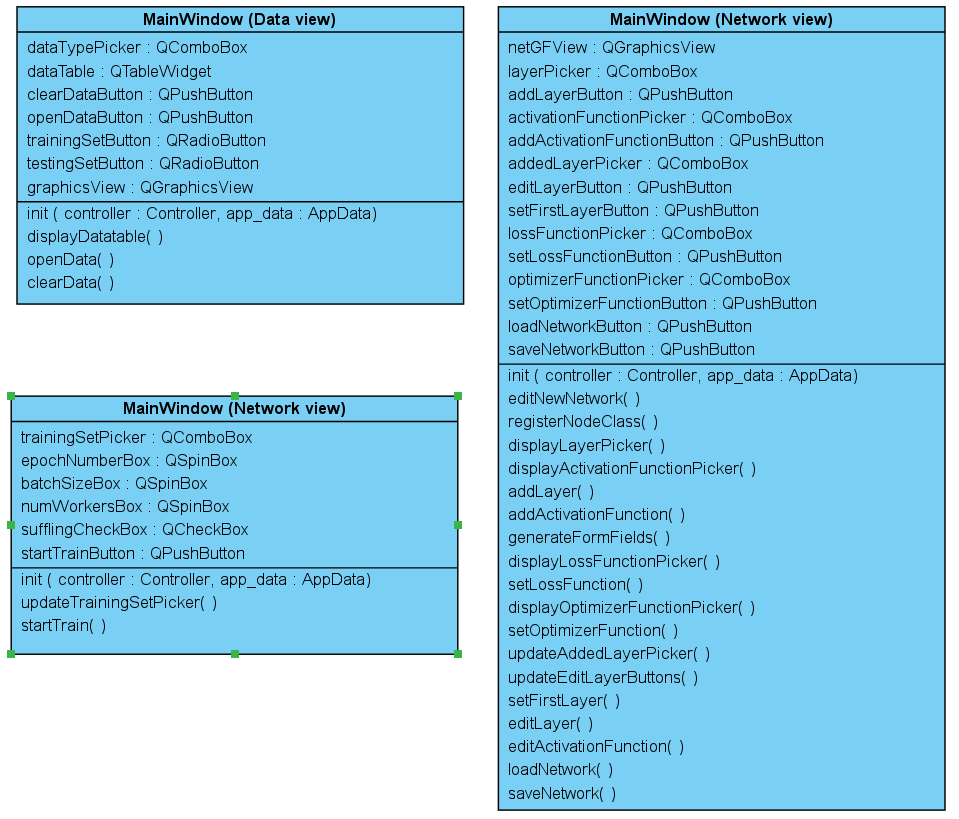
\includegraphics[scale=0.5]{figures/ViewDiagram.png}
    \caption{View class diagram \\ These are all \textbf{in the same class} (MainWindow), we just separated its content to clarify our explanation}
  \end{figure}

\begin{figure}[h!]
    \centering 
    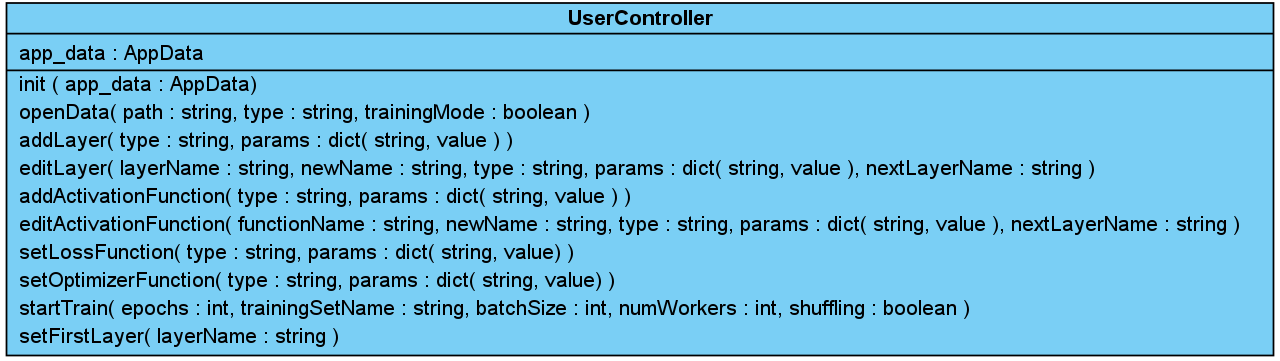
\includegraphics[scale=0.4]{figures/ControllerDiagram.png}
    \caption{Controller class diagram}
  \end{figure} 

% Architecture of the Application
%We need to describe Architecture of the Application as soon as its completed.
%for the moment it not completed
\vfill

\newpage
~
\newpage
%%%%%%%%%%%%%%%%%%%%%%%%%%%%%%%%%%%
\section{External Libraries}
\subsection{PyQT4}
Our application was mainly developed with PyQT4 a Python module wich allow usage of QTDesigner (version 4). QT designer is a graphical tools that let developer build Graphical Interfaces. At the opening, developer as the choice about the type of window he want to begin with: 

\begin{figure}[h!]
    \centering 
    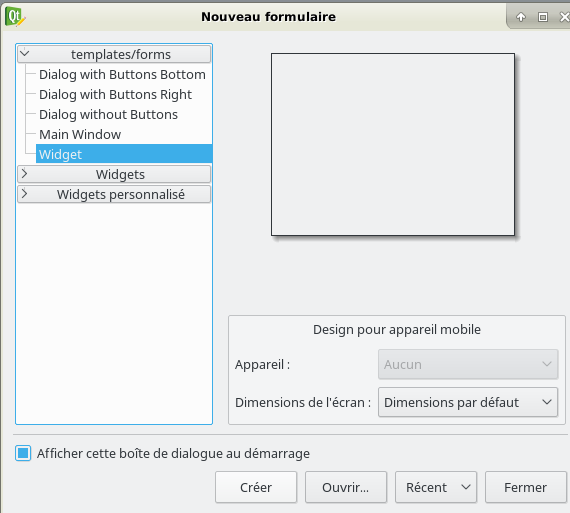
\includegraphics[scale=0.5]{figures/qt1.png}
    \caption{New form}
  \end{figure}

In our case, we chose to start with a blank "Main Window". This setting generate us our QMainWindow Class wich contains all of our widgets, layouts, buttons, graphics view, menu and status bar. 

\begin{figure}[h!]
    \centering 
    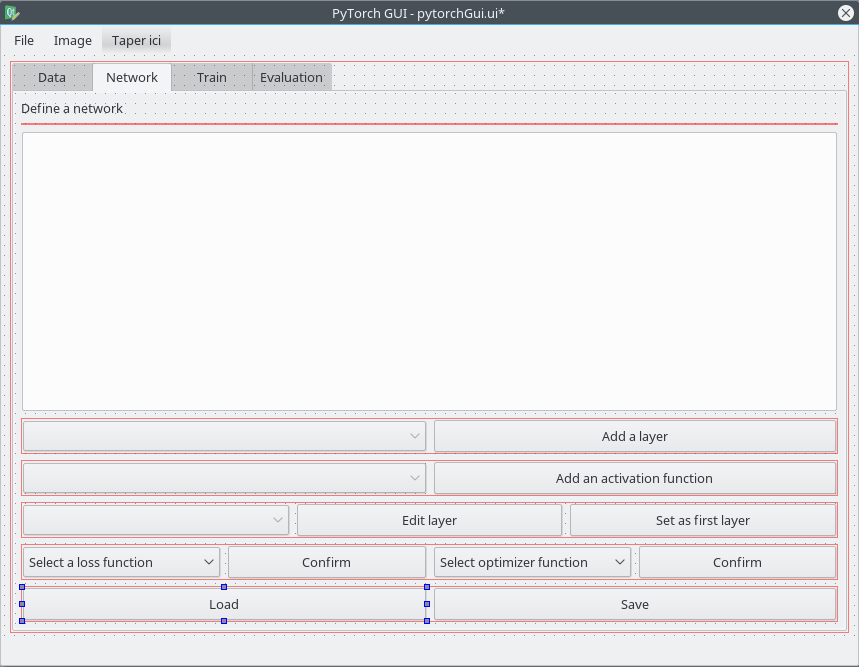
\includegraphics[scale=0.4]{figures/guirep.png}
    \caption{Component assembly in the Main Window}
  \end{figure}

For each of this objects, their classes are automatically generated and can be available in the "Main Window" attributes.  

\begin{figure}[h!]
    \centering 
    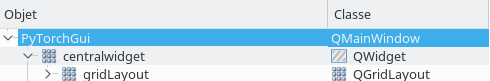
\includegraphics[scale=0.5]{figures/loadqt.png}
    \caption{Class representation of a "Load" button in QT Designer}
  \end{figure}
  
Signals and sloats are used for communication between objects, it's a central feature of Qt. All of our buttons are connected with functions. 

\subsubsection{Other libraries}
We will use some libraries that will ease us the task. Those libraries might change over the progress of our project :
\begin{itemize}
    \item qtnodes: qtnodes is a library that helped us to do the Node graph visualization and editing with PySide.
    \item PySide: A Python binding of Qt.
    \item Plotly: Using this library could be very useful. It can indeed provide a lot of graphical features, like plotting data, and generating graphs.
    \item Numpy: Numpy is an extension to the Python language, which allows to manipulate matrices and multidimensional arrays, and to use a variety of mathematical operations on it. Numpy is already integrated to PyTorch.
    \item Matplotlib: Plotting library for Python used to build and display graphs.
    \item Pydot: Python interface to Graphviz's Dot.
    \item Networkx: A python library for studying graphs and networks.
    \item Tqdm : Library used for display progress bar on terminal while training or evaluation of the neural network is in progress.
    \item SetupTools: It's a package development process library designed to facilitate packaging Python projects by enhancing the Python standard library distutils.
    \item Pandas: Library used for data manipulation and analysis.
    \item Appdirs: A small Python module for determining appropriate platform-specific directories.
\end{itemize}

\subsubsection{Utilities}

\begin{itemize}
    \item Version control system (VCS)
        As we work as a group and not individually on totally independent tasks, we have to use a VCS. Since we all know GitHub, we chose to use this simple VCS.
\end{itemize}

\begin{itemize}
    \item UML designer :
    \begin{itemize}
        \item VisualParadigm Online
        \item ArgoUML
    \end{itemize}
\end{itemize}
To clarify what we had to do to and move forward on the project, we needed to make a UML diagram. We first worked on VisualParadigm Online since we can all modify it then we finished it on ArgoUML.

%%%%%%%%%%%%%%%%%%%%%%%%%%%%%%%%%%%%
\subsection{Loading of the UI}
A really interesting feature of PyQT to facilitate the development of graphical interface is the ability to load a \textbf{.ui} file in the application. This file contains all the graphical structure of our application. It can be edited manually, but most importantly it can be created and edited from the application \textbf{QT Designer}. Therefore, with a practical interface, we can place all the graphical elements of our application, and place them into layouts. Layouts allow us to organize the display elements in an organized and aligned way. We can parameter all the fields, as well are their names. This kind of loading makes the development of this type of application easier and more flexible, since we don't have to directly modify code in order to edit most of the view elements.
\newline Once this file is loaded in our main window class, we have access to all the field with the corresponding variable name we chose when creating the UI file, and we can set values, as well as creating events, to program interaction with the user.
\begin{figure}[!h]
    \centering 
    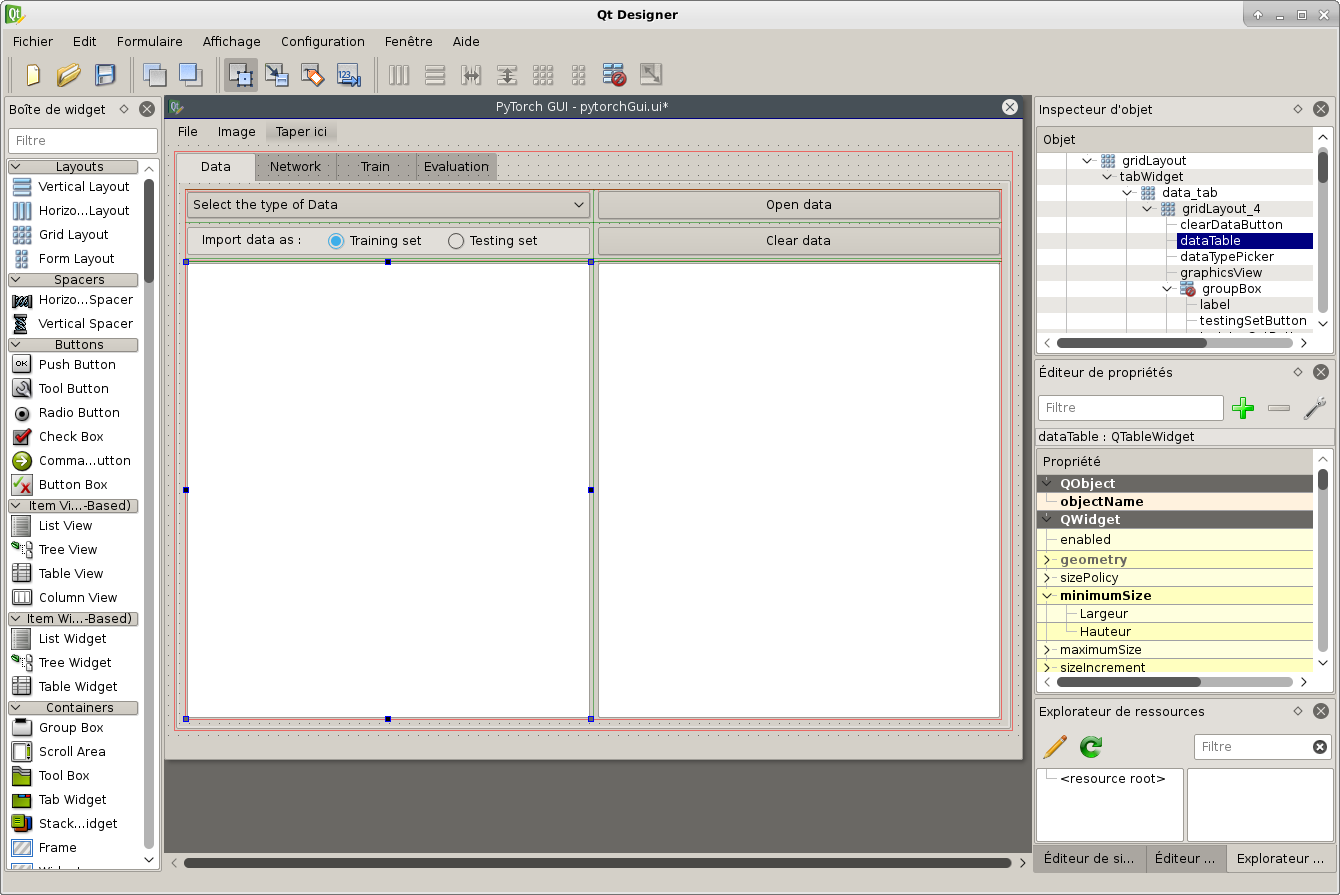
\includegraphics[scale=0.35]{figures/qt_designer.png}
    \caption{A screenshot of the QT Designer application}
\end{figure}
\subsection{Organisation of the network as a graph}
The main idea of a neural network is to be able to execute it by computing its layers in a certain order. This means layers follow each other until there is no \textbf{next layer}.
\subsubsection{Implementation}
To implement this graph in our code, we started by adding a python dictionary in our Network class. This dictionary is called \textbf{LayerList}, and it contains all the layers added in the network. We also have a second dictionary called \textbf{ActivationFunctionList} which contains all the added activation functions. 
\newline\textbf{Note :} both of these dictionaries contain entries to the type \textbf{Layer}, as in fact an activation function \textbf{is a layer}. We just decided to separate them in two different dictionaries, to facilitate the implementation of our graphical interface.
\newline Then, after adding the dictionaries to store our layer, we have to link layers between each other. To do so, we thought about a few possibilities. One of them was to create another dictionary, which would contain pairs of layers, which would mean they follow each other.
\newline To facilitate the iteration through our graph, we instead decided to set an attribute called \textbf{nextLayer} in our layers. That way, we can directly get the layer that follows the layer we just computed.
\begin{figure}[]
    \centering 
    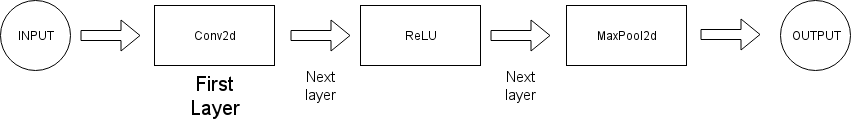
\includegraphics[scale=0.5]{figures/simple_graph.png}
    \caption{An example of a graph we can create with our current implementation}
\end{figure}
\subsubsection{Possible improvement : parallel execution}
A possible improvement we discussed about for our graph was to implement a way to execute multiple chains of layers at the same time. This happens to be useful in specific cases. To implement this we would have to create, among other things, a list of \textbf{first layers}, which would all take a copy on the input data, to execute them in parallel, and to make them merge into other layers, in order to have \textbf{only one output} at the end.
\begin{figure}[]
    \centering 
    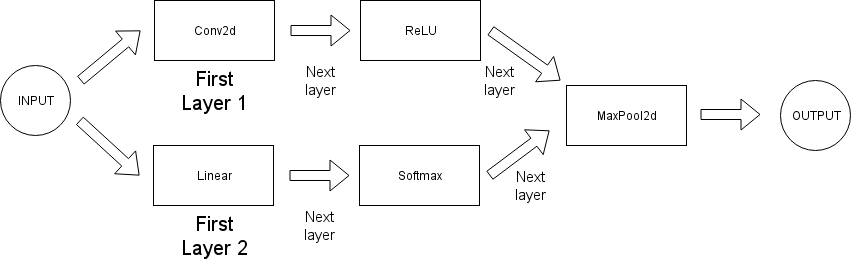
\includegraphics[scale=0.5]{figures/dual_graph.png}
    \caption{An example of a graph we could create by implementing parallel execution}
\end{figure}
\subsection{Usage of JSON files to store data}
\subsubsection{Why we used this format}
To be used as intended, our application has to store data on the disk.
\newline To begin, we have to store default values which are necessary to load our application at the beginning. These values are :
\begin{itemize}
    \item Available layer types in PyTorch, their parameters, the type of these parameters, as well as their default value
    \item Available activation functions (same thing)
    \item Available optimizer functions (same thing)
    \item Available loss functions (same thing)
\end{itemize}
We need all these informations, in order to display them to the user, and to allow them to choose a function or a layer, and parameter it in relation to the parameters accepted by PyTorch.
\newline In addition to that, we also have to be able to store the network created by the user. When the user wants to save the network he created, we have to generate a file which will describe all the structure of our network. Our application also has to allow the user to load a previously saved network from a file. Since this structure is a graph, we need a file structure which will allow us to easily describe its nodes and their relations.

Consequently, to fulfill all these needs, we needed a file format which would allow us to store data with a system of nodes. To do this, we had two main options : the XML format, and the JSON format. We decided to use a \textbf{JSON file format} to store our data, and the reasons for this choice are :
\begin{itemize}
    \item It is easier to parse than XML. A single line of code is needed to convert the content of the file to a python dictionary.
    \item It is lighter. The file takes less place, because there is no end-tag for each value. This is clearly valuable for us, since we have a great amount of default PyTorch functions to parse, it makes the file easier to read, and to modify.
\end{itemize}
\subsubsection{How we organized our JSON files to store default functions}
To store the default types of layers and functions available in PyTorch, we decided to organize our file as shown on the picture. We have a root which contains entries, and their names are the names of the associated functions in PyTorch. The values of these entries are other entries, which represent the different parameters of the function. The keys of these entries are the names of the parameters. The values are a \textbf{type} value, which allows our interface to know which type of field to display, and a \textbf{default} value, which contains the default value of this parameter, if there is one.
\newline \textbf{Note :} We based all our knowledge for these information on the official PyTorch documentation.
\begin{figure}[]
    \centering 
    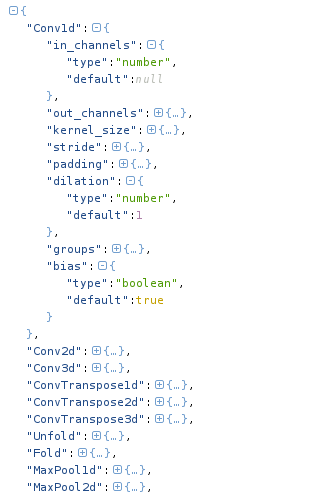
\includegraphics[scale=0.7]{figures/default_layer_types.png}
    \caption{A parsing of our JSON file for storing available layers in PyTorch}
\end{figure}

\subsubsection{How we load these default functions in our application}
To load these default functions, we have to parse the JSON file, and load the data in Python.
To do so, we created a class named \textbf{FunctionDatabase}. This class is responsible for loading all the default functions, by loading the content of the JSON file, and putting it into a python Ordered Dictionary. This dictionary will contain other dictionaries, which describe all the available parameters for the corresponding function. Default python dictionaries are not ordered, which means that by loading our default parameters to display them in the application, they might not appear in the right order. That's the reason why we used an OrderedDict, instead of a regular python dictionary. That way, all our available layers and functions, as well as their parameters will always be displayed in the same order, that means the order in which they have been written in the file.
\newline We use \textbf{a total of four FunctionDatabase}. One for the layers, one for the activation functions, one for the loss functions, and one for the optimizer functions. They are all stored in the \textbf{AppData} class, so they can be called and displayed from the view.
The corresponding JSON files are loaded once at the start of the application, then we never use them again.

\subsubsection{How we organized our JSON files to save and load created networks}
In order to store a created network, we also created our own format.
A way to save and load a network already exists in PyTorch. But it doesn't fit our needs. Firstly, it's encrypted in a way that it is only readable by PyTorch, so that a user can't read it and modify it manually. Also, it doesn't allow us to save the order of execution of our layers, which is a key part of how we designed our networks.
These are the reasons why we decided to, once again, create our own format.
\begin{figure}[]
    \centering 
    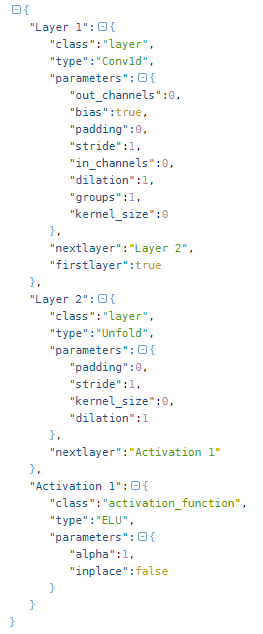
\includegraphics[scale=0.7]{figures/saved_network.png}
    \caption{A parsing of our JSON file for storing a saved network}
\end{figure}
\newline As you can see of the picture, our saved file is organized like this :
\begin{itemize}
    \item The root contains keys, which are the names of the different layers (or activation functions).
    \item Each of them contains information about the layer : its \textbf{class} ("layer" or "activation function"), its \textbf{type}, and its \textbf{parameters}.
    \item We also added a field containing the name of the \textbf{next layer}. This allows us to save our network \textbf{as a graph}.
    \item Lastly, we add an optional field named \textbf{firstlayer}, which tells us if the layer is the first layer of the network. It means that when training the network, it will start by computing this layer, and then the others.
\end{itemize}
\subsubsection{How we save a network to a JSON file}
In order to save our network to the JSON format, we first need to create the dictionary that will represent it. As always, we create an Ordered Dictionary, thus we can save everything in a predictable order.
\newline In order to store these information in the dictionary, we start by iterating through all the added layers, and we save them with the class "layer", their type, their parameters, the name of their next layer (if they have one), and a "firstLayer" value if it is the first layer of the graph. Then, we do the same by iterating through the added activation functions. The only difference here is that an activation function cannot be the first layer, so we put this possibility aside.
\newline When we finished to put the data we want to store in the dictionary, we just dump it directly to the JSON file.
\subsubsection{How we load a network from a JSON file}
The loading of a network from a json file works as follows :
\begin{enumerate}
    \item We clear the list of layers, and the list of activation functions, because we want to load a new network, without the layers from the old one
    \item We parse the json file, by converting it into an Ordered Dictionary
    \item We iterate through every node, and we create a Layer from the information stored in it (name, type, parameters).
    \item If the class is "layer", we add it to the layer list, and we check if it is the first layer of the network. If the class is "activation\_function", we add it to the activation function list.
    \item Once all our layers and functions are added to the lists, we iterate again through every node, to check which layer goes after the other, and we update these information on what we added before, to reconstitute our graph.
\end{enumerate}
\subsubsection{Loading of layer types and functions types in the view}
By using the different \textbf{FunctionDatabase} we loaded at the starting of the app, the view begins by loading the different layer types, activation function types, loss function types and optimizer function types in combo boxes. That way, the user can select the desired type, and initiate actions related to the selected type by clicking on the related buttons.
\subsubsection{Generating forms to add and edit network layers and functions}
When the user wants to parameter the network, he will want to set the different parameters of functions and layers. To do so, we generate dynamical forms, which parameters vary according to the type selected by the user. We take into account the type of parameter to generate a relevant field. For example, the type "number" will generate a number selector, and the type "boolean" will generate a checkbox.
\begin{figure}[]
    \centering 
    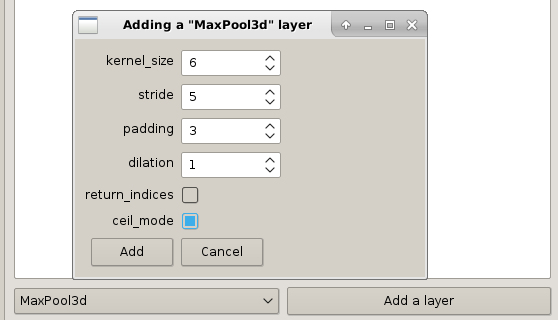
\includegraphics[scale=0.7]{figures/add_layer_form.png}
    \caption{An example of a generated form to add a layer to the network}
\end{figure}
\newline We generate this kind of forms for the following actions :
\begin{itemize}
    \item Adding a layer
    \item Adding an activation function
    \item Editing a layer
    \item Editing an activation function
    \item Setting the loss function
    \item Setting the optimizer function
\end{itemize}
If the user closes the form, nothing happens. If he validates it, the information is transmitted to the model, which creates (or modifies) the layer (or the function) with the corresponding parameters.
\newline When editing a layer or an activation function, two fields are added to the original parameters. These two fields are a text input for the name of the layer/function, and a combo box, which allows the user to select the next layer. It means that after the currently edited layer has been computed, it will then compute the layer selected in this field. By default, its value is \textbf{None}, so in this case the computation will stop here.